\section{6. Research, Testing, Evidence, and Release
Operations}\label{research-testing-evidence-and-release-operations}

This section points to the areas that prove the repo is not only broad,
but also inspectable and iterated with evidence.

\subsection{6.1 Research studies and option
papers}\label{research-studies-and-option-papers}

This subsection gathers the research material that sits behind
implementation choices and public examples.

The
\href{https://github.com/chris-page-gov/mcp-geo/tree/fe862910da246ca77f374cfbe484985f5df4d316/research}{research/}
directory is the long-horizon evidence surface behind the runtime. It
includes the
\href{https://github.com/chris-page-gov/mcp-geo/tree/fe862910da246ca77f374cfbe484985f5df4d316/research/From\%20Apps\%20to\%20Answers\%20-\%20Connecting\%20Public\%20Sector\%20Data\%20to\%20AI\%20with\%20MCP}{From
Apps to Answers research package}, the
\href{https://github.com/chris-page-gov/mcp-geo/tree/fe862910da246ca77f374cfbe484985f5df4d316/research/Deep\%20Research\%20Report}{Deep
Research Report set}, the
\href{https://github.com/chris-page-gov/mcp-geo/tree/fe862910da246ca77f374cfbe484985f5df4d316/research/map_delivery_research_2026-02}{map-delivery
research pack}, and the
\href{https://github.com/chris-page-gov/mcp-geo/tree/fe862910da246ca77f374cfbe484985f5df4d316/research/ons_dataset_selection}{ONS
dataset-selection work}. This is where design reasoning is preserved
before it is compressed into code or reports.

Where to go:
\href{https://github.com/chris-page-gov/mcp-geo/tree/fe862910da246ca77f374cfbe484985f5df4d316/research}{research/},
\href{https://github.com/chris-page-gov/mcp-geo/tree/fe862910da246ca77f374cfbe484985f5df4d316/research/From\%20Apps\%20to\%20Answers\%20-\%20Connecting\%20Public\%20Sector\%20Data\%20to\%20AI\%20with\%20MCP}{From
Apps to Answers research package},
\href{https://github.com/chris-page-gov/mcp-geo/tree/fe862910da246ca77f374cfbe484985f5df4d316/research/Deep\%20Research\%20Report}{Deep
Research Report},
\href{https://github.com/chris-page-gov/mcp-geo/tree/fe862910da246ca77f374cfbe484985f5df4d316/research/map_delivery_research_2026-02}{map-delivery
research}, and
\href{https://github.com/chris-page-gov/mcp-geo/tree/fe862910da246ca77f374cfbe484985f5df4d316/research/ons_dataset_selection}{ONS
dataset selection}.

\subsection{6.2 Tests, evaluation harnesses, and benchmark
packs}\label{tests-evaluation-harnesses-and-benchmark-packs}

This subsection explains where the repo proves behavior, not just
intent.

The
\href{https://github.com/chris-page-gov/mcp-geo/tree/fe862910da246ca77f374cfbe484985f5df4d316/tests}{tests/}
tree covers the runtime broadly, but the most revealing concentrated
evidence sits in
\href{https://github.com/chris-page-gov/mcp-geo/tree/fe862910da246ca77f374cfbe484985f5df4d316/tests/evaluation}{tests/evaluation/},
\href{https://github.com/chris-page-gov/mcp-geo/tree/fe862910da246ca77f374cfbe484985f5df4d316/playground/tests}{playground/tests/},
and the generated benchmark artifacts under
\href{https://github.com/chris-page-gov/mcp-geo/tree/fe862910da246ca77f374cfbe484985f5df4d316/data/benchmarking}{data/benchmarking/}.
Pair those with
\href{https://github.com/chris-page-gov/mcp-geo/blob/fe862910da246ca77f374cfbe484985f5df4d316/docs/evaluation.md}{docs/evaluation.md}
and the
\href{https://github.com/chris-page-gov/mcp-geo/blob/fe862910da246ca77f374cfbe484985f5df4d316/docs/reports/README.md\#L66-L71}{stakeholder
evaluation reports} when you need to see how the repo turns tests into
public evidence.

Where to go:
\href{https://github.com/chris-page-gov/mcp-geo/tree/fe862910da246ca77f374cfbe484985f5df4d316/tests}{tests/},
\href{https://github.com/chris-page-gov/mcp-geo/tree/fe862910da246ca77f374cfbe484985f5df4d316/tests/evaluation}{tests/evaluation/},
\href{https://github.com/chris-page-gov/mcp-geo/tree/fe862910da246ca77f374cfbe484985f5df4d316/playground/tests}{playground/tests/},
\href{https://github.com/chris-page-gov/mcp-geo/tree/fe862910da246ca77f374cfbe484985f5df4d316/data/benchmarking}{data/benchmarking/},
and
\href{https://github.com/chris-page-gov/mcp-geo/blob/fe862910da246ca77f374cfbe484985f5df4d316/docs/evaluation.md}{docs/evaluation.md}.

\begin{figure}
\centering
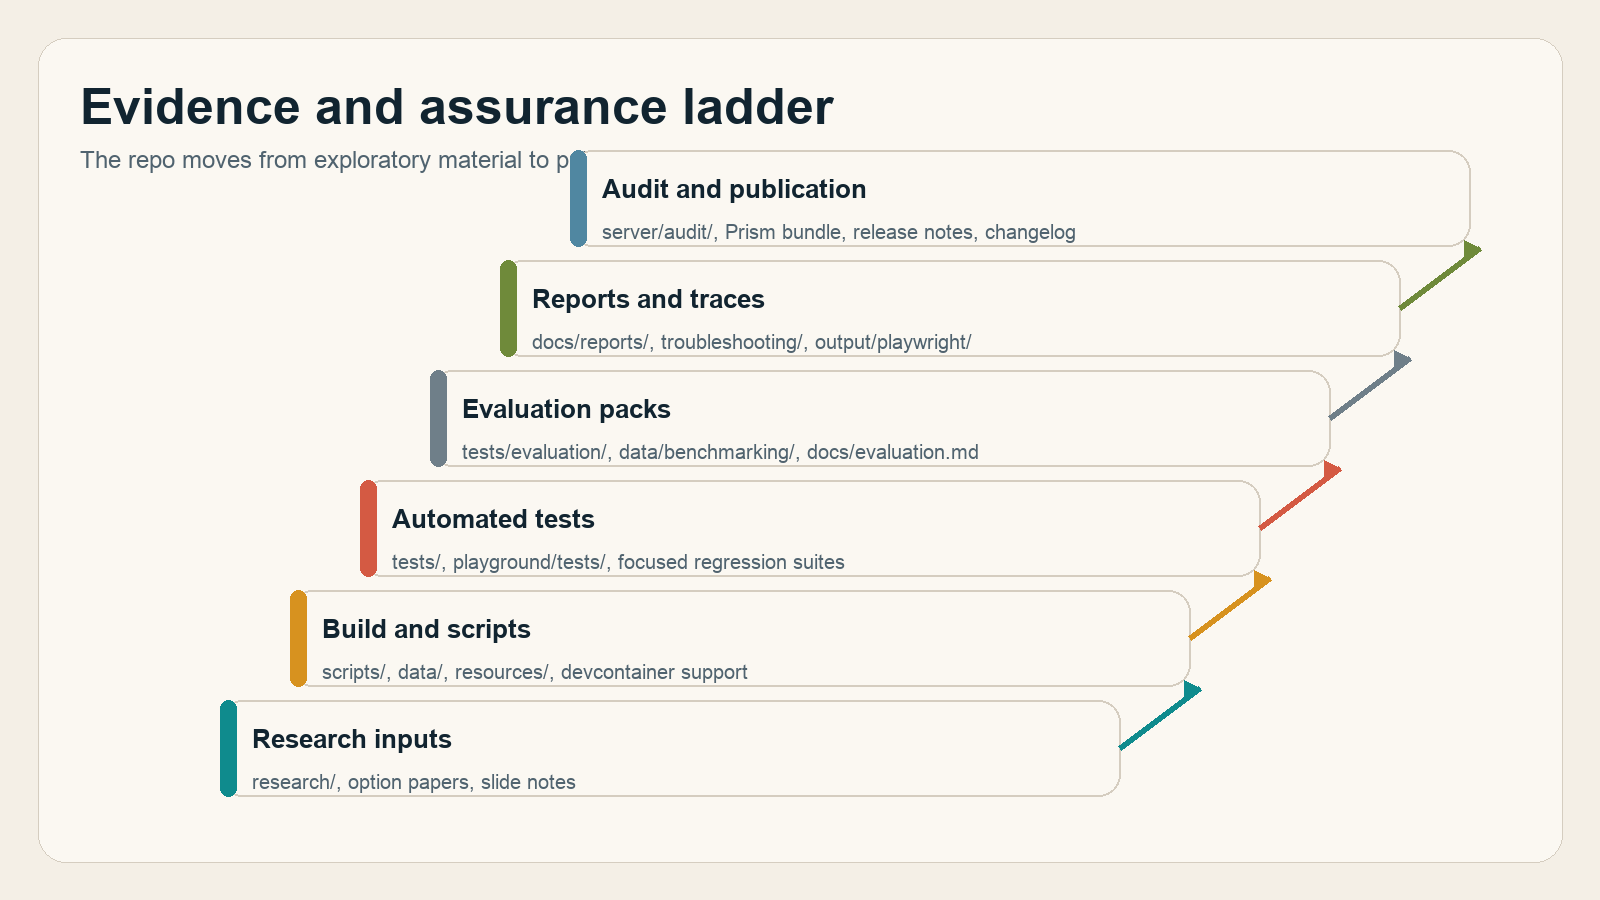
\includegraphics[width=0.96\linewidth,height=\textheight,keepaspectratio,alt={Figure F06. Evidence and assurance ladder}]{figures/f06_evidence_assurance_ladder.png}
\caption{Figure F06. Evidence and assurance ladder}
\end{figure}

Figure F06 makes the assurance story visible: research feeds tests,
tests feed evaluation, and evaluation feeds reports and audit material.

\subsection{6.3 Release, CI, troubleshooting, and maturity
signals}\label{release-ci-troubleshooting-and-maturity-signals}

This subsection groups the files that show how work is stabilized,
published, and investigated when something goes wrong.

The repo's maturity signals are distributed across
\href{https://github.com/chris-page-gov/mcp-geo/blob/fe862910da246ca77f374cfbe484985f5df4d316/.github/workflows/ci.yml}{\texttt{.github/workflows/ci.yml}},
\href{https://github.com/chris-page-gov/mcp-geo/blob/fe862910da246ca77f374cfbe484985f5df4d316/CHANGELOG.md}{CHANGELOG.md},
\href{https://github.com/chris-page-gov/mcp-geo/tree/fe862910da246ca77f374cfbe484985f5df4d316/RELEASE_NOTES}{RELEASE\_NOTES/},
\href{https://github.com/chris-page-gov/mcp-geo/blob/fe862910da246ca77f374cfbe484985f5df4d316/docs/troubleshooting.md}{docs/troubleshooting.md},
the
\href{https://github.com/chris-page-gov/mcp-geo/tree/fe862910da246ca77f374cfbe484985f5df4d316/troubleshooting}{troubleshooting/}
directory, and the durable planning pair of
\href{https://github.com/chris-page-gov/mcp-geo/blob/fe862910da246ca77f374cfbe484985f5df4d316/CONTEXT.md}{CONTEXT.md}
and
\href{https://github.com/chris-page-gov/mcp-geo/blob/fe862910da246ca77f374cfbe484985f5df4d316/PROGRESS.MD}{PROGRESS.MD}.
Read this cluster when the question is about release readiness,
operational history, or why a prior experiment failed.

Where to go:
\href{https://github.com/chris-page-gov/mcp-geo/blob/fe862910da246ca77f374cfbe484985f5df4d316/.github/workflows/ci.yml}{\texttt{.github/workflows/ci.yml}},
\href{https://github.com/chris-page-gov/mcp-geo/blob/fe862910da246ca77f374cfbe484985f5df4d316/CHANGELOG.md}{CHANGELOG.md},
\href{https://github.com/chris-page-gov/mcp-geo/tree/fe862910da246ca77f374cfbe484985f5df4d316/RELEASE_NOTES}{RELEASE\_NOTES/},
\href{https://github.com/chris-page-gov/mcp-geo/blob/fe862910da246ca77f374cfbe484985f5df4d316/docs/troubleshooting.md}{docs/troubleshooting.md},
\href{https://github.com/chris-page-gov/mcp-geo/tree/fe862910da246ca77f374cfbe484985f5df4d316/troubleshooting}{troubleshooting/},
\href{https://github.com/chris-page-gov/mcp-geo/blob/fe862910da246ca77f374cfbe484985f5df4d316/CONTEXT.md}{CONTEXT.md},
and
\href{https://github.com/chris-page-gov/mcp-geo/blob/fe862910da246ca77f374cfbe484985f5df4d316/PROGRESS.MD}{PROGRESS.MD}.

\begin{figure}
\centering
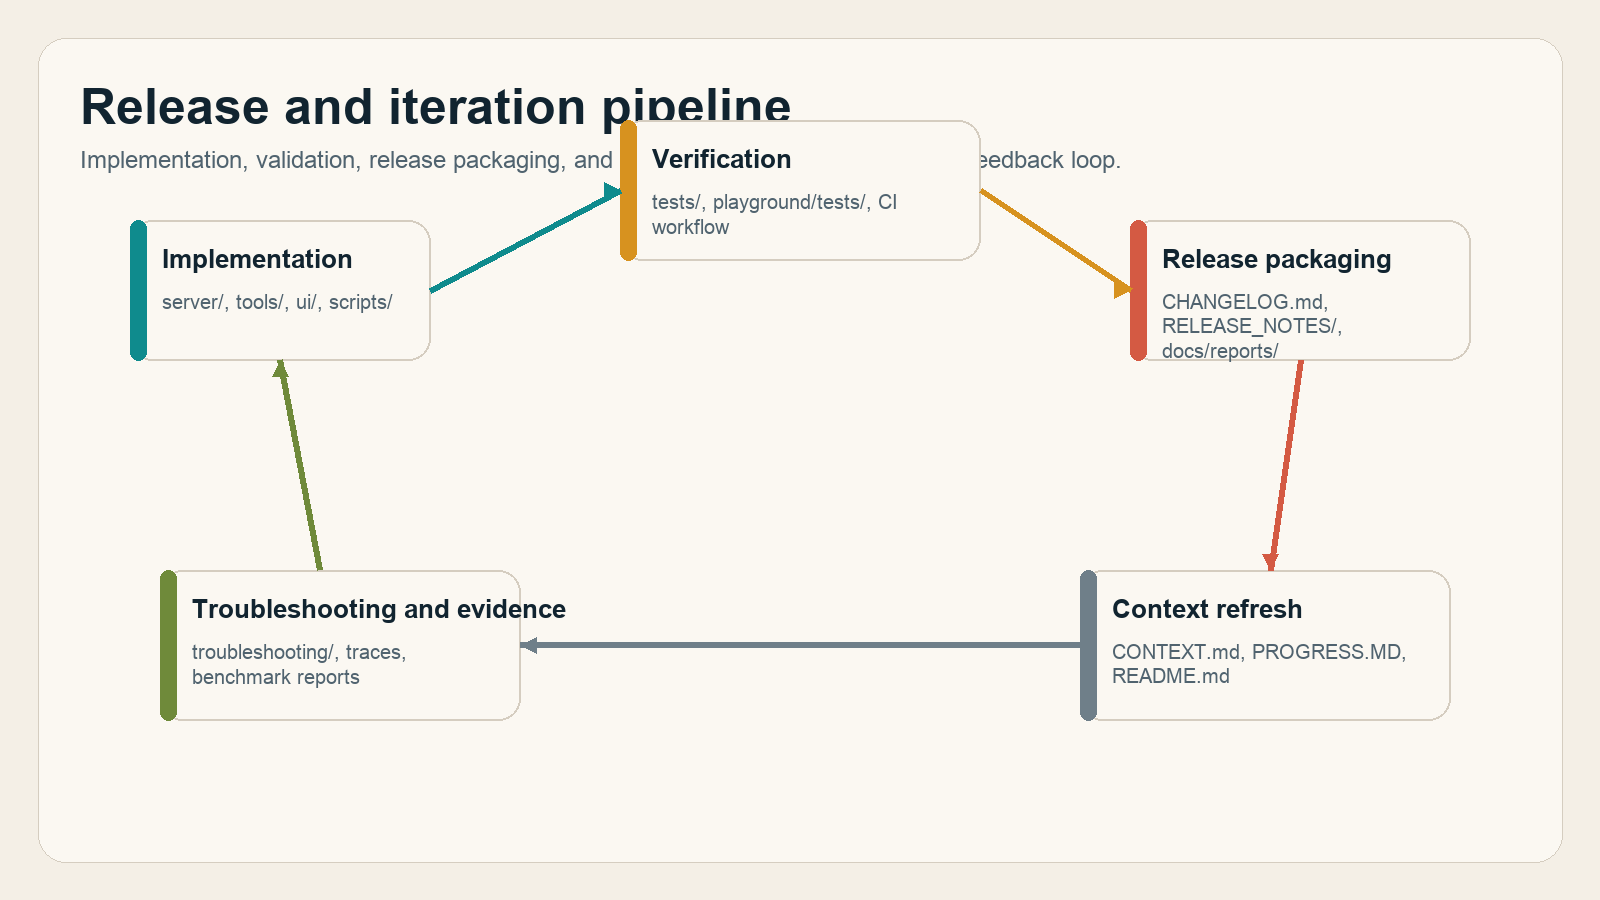
\includegraphics[width=0.96\linewidth,height=\textheight,keepaspectratio,alt={Figure F07. Release and iteration pipeline}]{figures/f07_release_iteration_pipeline.png}
\caption{Figure F07. Release and iteration pipeline}
\end{figure}

Figure F07 shows how implementation, verification, release packaging,
and documentation updates loop back into each other.
